% Preamble
\documentclass{article}

% Packages
\usepackage[T1]{fontenc} % Fontes T1
\usepackage[utf8]{inputenc} % Input UTF8
\usepackage[backend=biber, style=ieee]{biblatex} % para usar bibliografia
\usepackage{csquotes}
\usepackage[portuguese]{babel} %Usar língua portuguesa
\usepackage{blindtext}
\usepackage{graphicx} % Gerar texto automaticamente
\usepackage{geometry}
\usepackage{float}
\usepackage{indentfirst}
\usepackage[printonlyused]{acronym}
\usepackage{ragged2e}
\usepackage{textcomp}

% Document
\begin{document}
    % Define keybinds
    \def\title{\textbf{MÁQUINA DE FAZER PÃO}}
    \def\authors{João Bastos (113470), Rúben Gomes(113435)}
    \def\contacts{(113470) joaop.bastos@ua.pt, (113435) rlcg@ua.pt}
    \def\department{Departamento de Eletrónica, Telecomunicações e Informática}
    \def\university{Universidade de Aveiro}
    \def\logo{ua.pdf}


    % Header
    \fancyhead{
        \begin{center}
            \includegraphics{\logo}\\
            \textbf{{\LARGE \title}}\\
            \vspace{2mm}
            \large Trabalho realizado por: \authors.\\
        \end{center}
    }

    % Introduction
    \section{Introdução}\label{sec:introducao}
        \par Este projeto visa a implementar uma máquina de fazer pão, que permita ao utilizador escolher o tipo de pão que pretende fazer. \ Para tal, é necessário que o programa tenha uma máquina de estados finitos que permita ao utilizador escolher o tipo de pão a ser fabricado facilmente, bem como adicionar tempo extra de cozedura e/ou tempo prévio de espera para iniciar a máquina.\\

        Para tornar este projeto possível, pretendemos implementar uma máquina de estados, e os seus componentes necessários em linguagem de \textit{hardware} \acs{vhdl} e desenvolvido no software Quartus\textregistered Prime, de forma a aplicar a matéria lecionada na cadeira de \acs{lsd}.

    % Architecture
    \section{Arquitetura}\label{sec:arquitetura}
        \par A arquitetura deste projeto é divisível em várias partes distintas, que, logicamente, são complementares para o resultado do projeto. \ Estas serão descritas abaixo da seguinte figura. \\

        \begin{figure}[H]
            \centering
            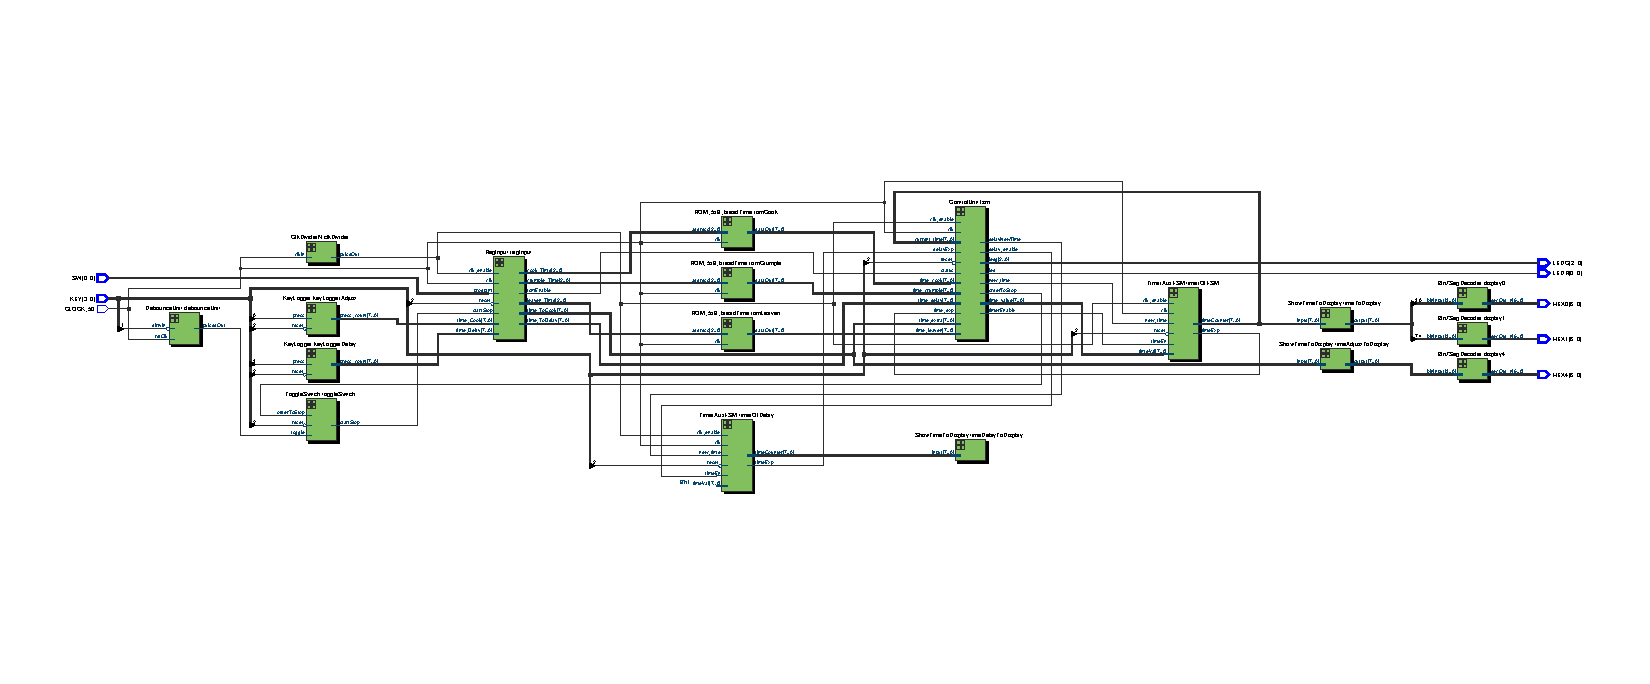
\includegraphics[scale=0.6]{BreadMachine}
            \caption{Figura representativa do \textit{top-level} do projeto}
            \label{fig:bread-machine}
        \end{figure}

    \begin{itemize}
        \item[\textbf{\textrightarrow}] \textbf{KeyLogger} - Este bloco é responsável por um simples registo de cliques em um dado botão, ou seja, ao clicar uma vez, é registado esse clique como uma unidade de tempo de espera ou extra.
        \item[\textbf{\textrightarrow}] \textbf{ToggleSwitch} - O componente ToggleSwitch é usado para começar/parar a máquina de pão a qualquer momento, simulando um \textit{switch}.
        \item[\textbf{\textrightarrow}] \textbf{ClkDividerN} - Este componente é responsável por dividir o sinal de \textit{clock} por um determinado valor, de forma a que seja enviado um puslo  de um certo valor de Hertz. \ Por motivos de estar em causa um temporizador, este tem de ser dividido de forma a gerar um pulso de 1 Hz.
        \item[\textbf{\textrightarrow}] \textbf{DebounceUnit} - Este componente é usado para controlar o uso de um botão. \ Um botão em uma FPGA manda centenas de sinais ao ser clicada. \ Ao usar este componente, é possível controlar o número de sinais enviados, de forma a que o botão seja ativado apenas uma vez, sem repetições.
        \item[\textbf{\textrightarrow}] \textbf{ROM\_5x8\_breadTime} - É uma memória que armazena 5 palavras de 8 bits, sendo cada palavra o tempo de um programa (como tempo de cozedura de pão rústico, por exemplo), que serão enviados para a State Machine(mais sobre a mesma na %TODO:referencia a state machine)
        \item[\textbf{\textrightarrow}] \textbf{} 
    \end{itemize}



    A arquitetura deste projeto é composta por uma máquina de estados finitos, composta por 6 estados diferentes, estes sendo:
    \begin{itemize}
        \item \textbf{STANDBY} - Este estado é o estado inicial da máquina. \ Por defeito, permite selecionar o programa que o utilizador pretende, adicionar tempo extra de cozedura ou adicionar tempo de espera total da máquina. \ Este estado será ativado quando o utilizador clica no botão de reset ou o pão a ser processado acaba o seu tempo de cozedura;
        \item \textbf{}
    \end{itemize}




    % Acronyms
    \newpage
    \section*{Acrónimos}
    \begin{acronym}
        \acro{vhdl}[VHDL]{Very High-Speed Integrated Circuit Hardware Description Language}
        \acro{lsd}[LSD]{Laboratório de Sistemas Digitais}
    \end{acronym}

    \begin{flushright}
        \today
    \end{flushright}
\end{document}